\documentclass[a4paper,11pt]{article}
%
% document setup, package import, etc.
%
%
% packages and settings for the worksheet files
%
\usepackage[bf,small]{titlesec}
\usepackage{graphicx}
\usepackage{amsfonts,amssymb,amsmath,fancyhdr}
%\usepackage{import} % needed for subimport
\usepackage{url}
\usepackage{paralist} % needed for compactenum
\usepackage{verbatim} % needed for varbatimiinput
\usepackage{shortlst}
\usepackage{siunitx}
%
%  page layout
%
\setlength{\textwidth}{175mm}
\setlength{\textheight}{240mm}
\setlength{\voffset}{-20mm}
\setlength{\hoffset}{-23mm}
\setlength{\parskip}{0pt}
\setlength{\parindent}{0pt}
\setlength{\footskip}{40pt}
\renewcommand{\baselinestretch}{1.2} \small\normalsize
%
%  Header/footer
%
\fancyhf{} % Clear all fields
\renewcommand{\headrulewidth}{0pt}
\renewcommand{\footrulewidth}{0pt}
\fancyfoot[L]{\footnotesize EMAT20920 2020-21}
\fancyfoot[C]{\footnotesize \thepage}
\fancyfoot[R]{\footnotesize COURSEWORK ASSESSMENT}
%
% Change list-making
%
\renewcommand{\theenumi}{\alph{enumi}}
\def\labelenumi{(\theenumi)}
\renewcommand{\theenumii}{\roman{enumii}}
\def\labelenumii{(\theenumii)}
%
% Change section headers
%
\titlelabel{Question \thetitle:\quad}
%
% First page header
%
\newcommand{\solutionsheader}[2]{
    \pagestyle{fancy}
    \begin{center}
      {\large Department of Engineering Mathematics}\\[3ex]
      \textbf{EMAT20920: Numerical Methods in MATLAB}\\[3ex]
      \textbf{#1}\\
      \textbf{#2}
    \end{center}}
%
% For formatting matlab code with listings
%
\usepackage{listings}
\usepackage{color}
\usepackage{textcomp}
\definecolor{listinggray}{gray}{0.9}
\definecolor{lbcolor}{rgb}{0.9,0.9,0.9}
\lstset{
    backgroundcolor=\color{lbcolor},
    numbers=none,
    numberstyle=\tiny,
    tabsize=4,
    rulecolor=,
    language=matlab,
    basicstyle=\scriptsize\ttfamily,
    upquote=true,
    aboveskip={1.5\baselineskip},
    columns=flexible,
    showstringspaces=false,
    extendedchars=true,
    breaklines=true,
    prebreak = \raisebox{0ex}[0ex][0ex]{\ensuremath{\hookleftarrow}},
    %frame=single,
    showtabs=false,
    showspaces=false,
    showstringspaces=false,
    identifierstyle=\ttfamily,
    keywordstyle=\color[rgb]{0,0,1},
    commentstyle=\color[rgb]{0.133,0.545,0.133},
    stringstyle=\color[rgb]{0.627,0.126,0.941},
    aboveskip=0pt,
    belowskip=2pt,
}
%
% shortcut commands
%
\newcommand{\matcmd}[1]{\colorbox{lbcolor}{\lstinline{#1}}}
\newcommand{\matlab}[1]{\texttt{#1}}
\renewcommand{\vec}[1]{\boldsymbol{#1}}
\newcommand{\order}{\mathcal{O}}

\newenvironment{listcomment}[1][1]{\framed\adjustwidth{-\dimexpr 
#1\leftmargin + \fontdimen2\font}{}}{\endadjustwidth\endframed}


\begin{document}

\solutionsheader{COURSEWORK ASSESSMENT}{Jake Bowhay (UP19056)}

All figures in this report have been saved using \verb*|saveFigPDF| function 
as it automatically resizes the paper to the correct size.
\lstinputlisting{../src/saveFigPDF.m}

\section{Root-finding}
\begin{enumerate}
	\item To find how many solutions each equation has in the given domain I 
	will rearrange all the equations to be equal to zero and then looks for 
	the zeros of the rearranged equations. As a corollary to the intermediate 
	value theorem, if a function is continuous and changes sign in a bracket 
	then that bracket must contain a zero. So I will plot each of the 
	rearranged equation and I look for appropriate brackets. I will use the 
	\verb*|pltFunc| function to plot the functions as it removes values 
	outside a defined limit which prevents MATLAB plotting discontinuous 
	functions as continuous. The limits can then be changed using the 
	property explorer to give a more useful plot.
	\lstinputlisting{../src/q1/pltFunc.m}
	\begin{enumerate}
		\item Rearranging $x^{4} = e^{-x} \cos(x)$ gives $f(x) = x^{4} - 
		e^{-x} \cos(x)$.
		\lstinputlisting{../src/q1/Q1a_i.m}
		\NoIndent{
			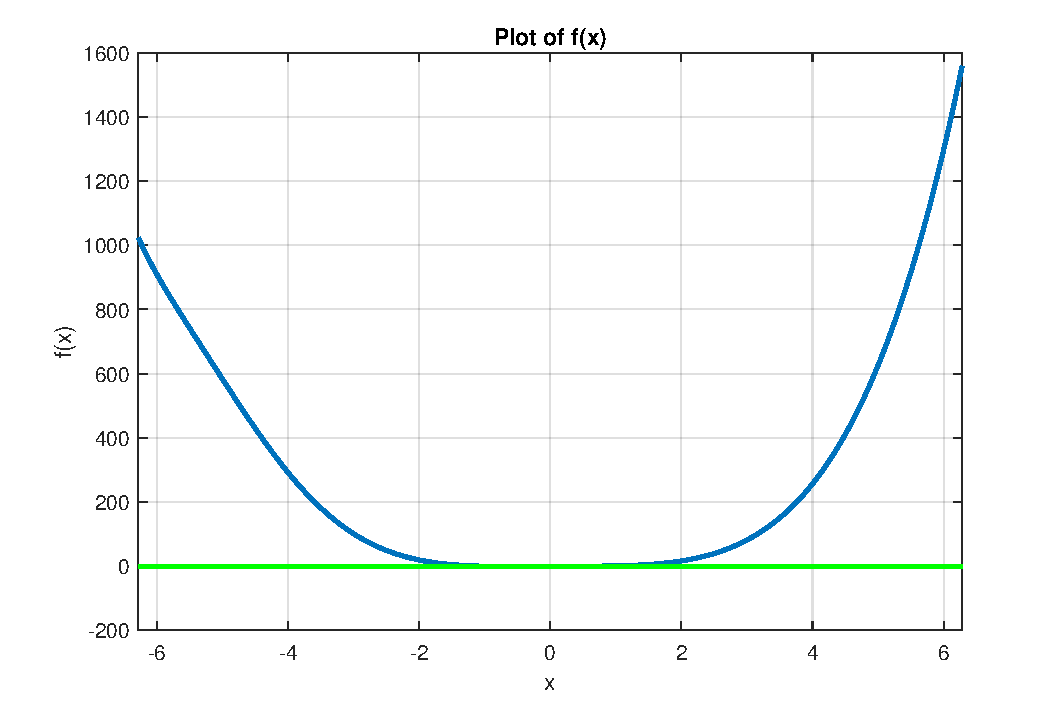
\includegraphics[scale=0.5]{images/Q1a_i.pdf}
			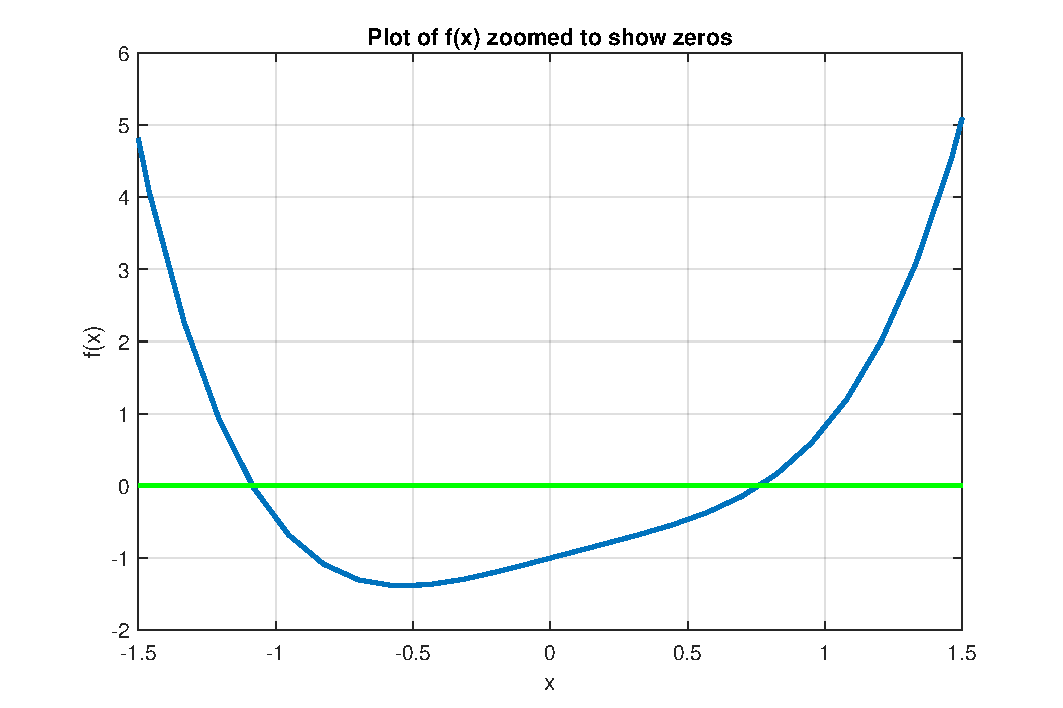
\includegraphics[scale=0.5]{images/Q1a_i_zoomed.pdf}
		}
			The second zoomed in plot shows there are two zeros in the given 
			domain. The first zero can be bracketed by the interval 
			$[-1.5,-1]$ as 
			$f(-1.5)=4.7455$ and $f(-1)=-0.4687$ so since the function is 
			continuous and there is a change of sign this bracket must 
			contain 
			a zero. Like wise the second root can be bracketed by the 
			interval $[0.5,1]$ 
			as $f(0.5)=-0.4698$ and $f(1)=0.8012$.
			
			
		\item Setting $f(x) = \frac{x^{3}}{\sin(x)} - 1$.
			\lstinputlisting{../src/q1/Q1a_ii.m}
		\NoIndent{
			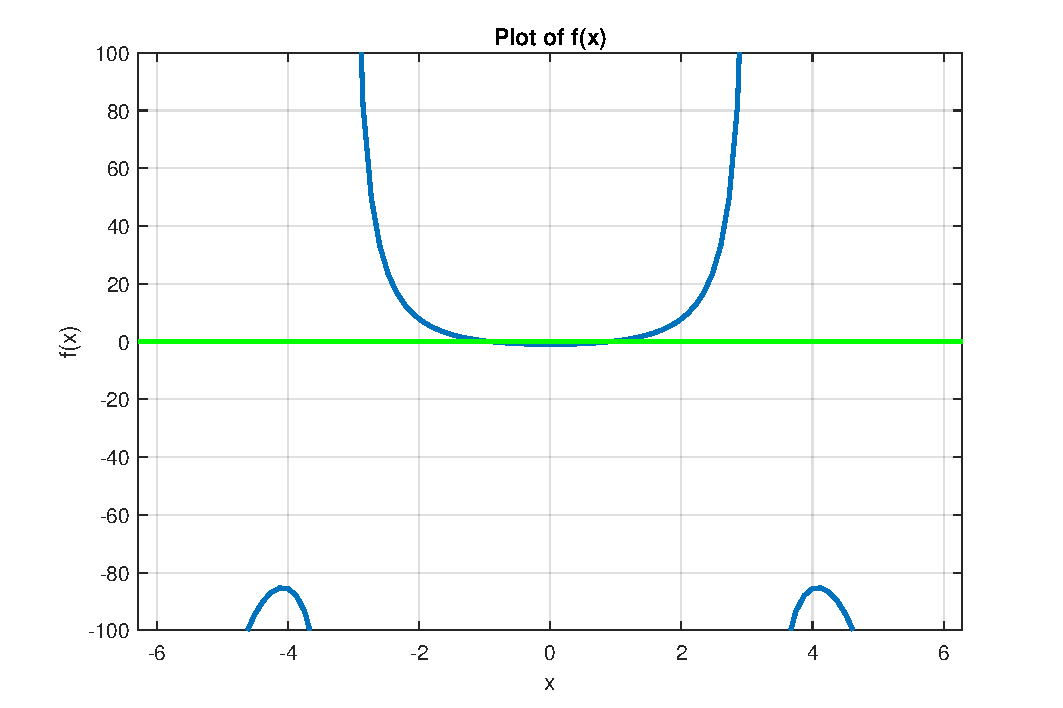
\includegraphics[scale=0.5]{images/Q1a_ii.pdf}
			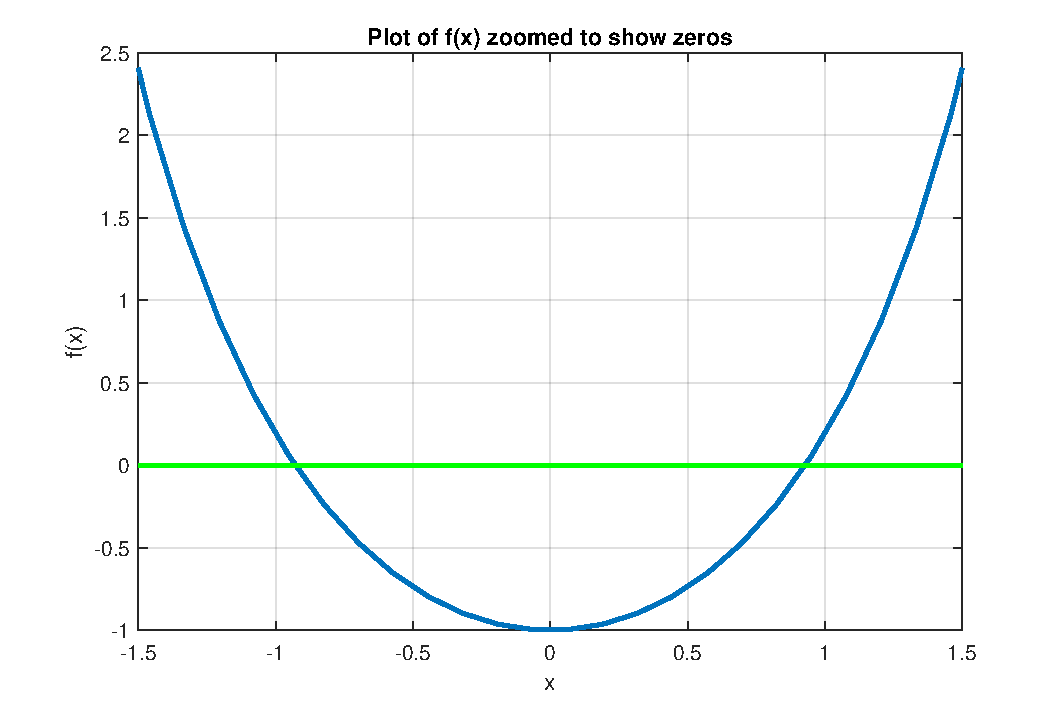
\includegraphics[scale=0.5]{images/Q1a_ii_zoomed.pdf}
		}
		The second plot show there are two roots. The first root can be 
		bracketed by the interval $[-1,-0.5]$ as $f(-1) = 0.1884$ 
		and 
		$f(-0.5)=-0.7393$ and $f(x)$ is continuous in this bracket. Likewise, 
		the second root can be bracketed by the interval $[0.5,1]$ as 
		$f(0.5)=-0.7393$ and 
		$f(1)=0.1884$.
		
		
		\item Rearranging $\cot(x) = \frac{25}{25x-1}$ gives $f(x) = \cot(x) 
		- \frac{25}{25x-1}$.
		\lstinputlisting{../src/q1/Q1a_iii.m}
		\begin{center}
			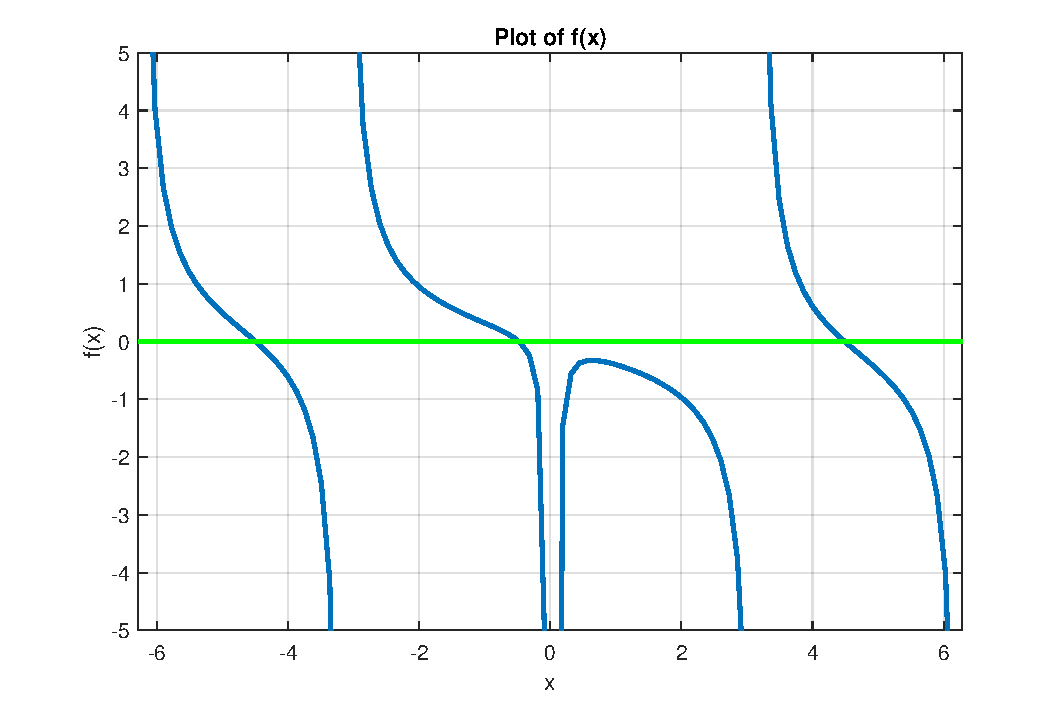
\includegraphics[scale=0.5]{images/Q1a_iii.pdf}
		\end{center}
		The plot shows that the equation has three solutions. The first can 
		be bracketed by the interval $[-5,-4]$ as $f(-5)=0.4942$ and 
		$f(-4)=-0.6162$. The 
		second solution can be bracketed by the interval $[-1,-0.1]$ as 
		$f(-1)=0.3194$ and 
		$f(-0.1)=-2.8238$. The third solution can be bracketed by the 
		interval $[4,5]$ as 
		$f(4)=0.6112$ and $f(5)=-0.4974$. $f(x)$ is continuous in each of the 
		bracketing intervals.
	
		\item Rearranging $4e^{-x^{2}/5} = cos(5x) + 2$ gives $f(x) = 
		4e^{-x^{2}/5} - cos(5x) - 2$.
		\lstinputlisting{../src/q1/Q1a_iv.m}
		\NoIndent{
		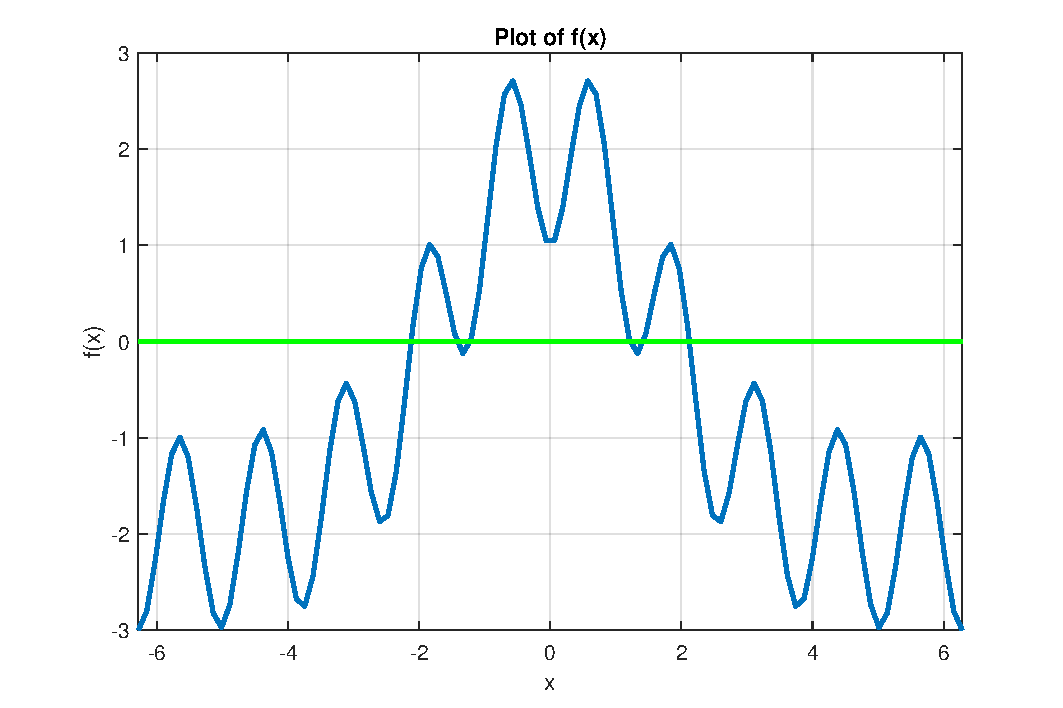
\includegraphics[scale=0.5]{images/Q1a_iv.pdf}
		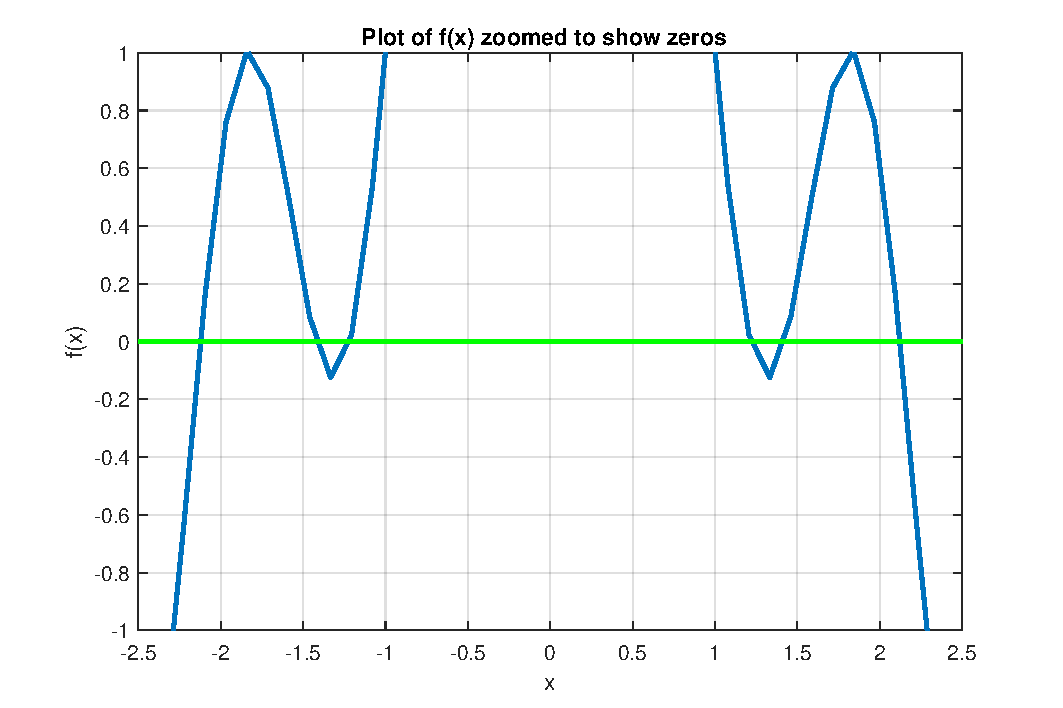
\includegraphics[scale=0.5]{images/Q1a_iv_zoomed.pdf}
		}
		The second plot shows that the equation has 6 solutions. The 
		bracketing intervals are shown in the table below.
		\begin{table}[!h]
			\centering
			\begin{tabular}{l|ll}
				$[a,b]$        & f(a)    & f(b)    \\ \hline
				$[-2.5,-2]$    & -1.8518 & 0.6364  \\
				$[-1.5,-1.25]$ & 0.2039  & -0.0730 \\
				$[-1.25,-1]$   & -0.0730 & 0.9913  \\
				$[1,1.25]$     & 0.9913  & -0.0730 \\
				$[1.25,1.5]$   & -0.0730 & 0.2039  \\
				$[2,2.5]$      & 0.6364  & -1.8518
			\end{tabular}
		\end{table}
	\end{enumerate}



	\item The bisection method used by calling the the \verb*|bisectRoot| 
	function.
	\lstinputlisting{../src/q1/bisectRoot.m}
	
	
	\begin{enumerate}
		\item Solutions to $f(x) = x^{4} - e^{-x} \cos(x) = 0 \  \ 
		x\in[-2\pi,2\pi]$.
		\lstinputlisting{../src/q1/Q1b_i.m}
		Note the two different tolerances since one root is an order of 
		magnitude larger so requires one less decimal place of accuracy to be 
		accurate to 8 significant figures.
		\begin{table}[!h]
			\centering
			\begin{tabular}{l|ll}
				$[a,b]$     & Root       & \# Iterations \\ \hline
				$[-1.5,-1]$ & -1.0843596 & 23           \\
				$[0.5,1]$   & 0.76221106 & 26          
			\end{tabular}
		\end{table}
	
	
		\item Solutions to $f(x) = \frac{x^{3}}{\sin(x)} - 1 = 0 \  \ 
		x\in[-2\pi,2\pi]$.
		\lstinputlisting{../src/q1/Q1b_ii.m}
		\begin{table}[!h]
			\centering
			\begin{tabular}{l|ll}
				$[a,b]$     & Root        & \# Iterations \\ \hline
				$[-1,-0.5]$ & -0.92862631 & 26            \\
				$[0.5,1]$   & 0.92862631  & 26           
			\end{tabular}
		\end{table}
	
	
		\item
	\end{enumerate}
\end{enumerate}


\end{document}
